\section{Experimental Results}
\label{sec:chromium-results}

\subsection{RQ1: Discerning flaky from fault triggering test failures when training on tests}

We trained a model on 69,159 passing tests, 910 fault-revealing tests and 8,857 flaky tests (unique tests).
Then, we evaluated it on 217,503 failures caused by flaky tests and 2,320 fault-triggering failures caused by fault-revealing tests. Table ~\ref{table:rq1} reports the obtained performance. Similar to the performance achieved by previous vocabulary-based models on other datasets, our model was able to reach high accuracy with a precision of 99.2\% and a recall of 98.9\%. However, we note a high false-positive rate. This is due to an important amount (76.2\%) of fault-triggering failures classified as flaky (FP). This is concerning: fault-triggering failures should not be misclassified as they reflect the existence of real faults. Overall, the MCC value is equal to 0.20, which is relatively low and shows that the model struggles (compared to random selection) to identify fault-triggering failures. 

\begin{table}[ht]
\caption{Vocabulary-based model performance for the prediction of \textit{flaky test failures vs fault-triggering failures} when trained on flaky vs non-flaky (fault-revealing and passing tests). Despite a high accuracy on flaky failures, the low MCC and high FPR show us that it remains challenging for the model to classify negative elements (in our case: fault-triggering failures)}
\label{table:rq1}
\centering
\begin{tabular}{c|c|c|c} 
 \toprule
 \textbf{Precision} & \textbf{Recall} & \textbf{MCC} & \textbf{FPR} \\ [0.5ex] 
 \midrule
 99.2\% & 98.9\% & 0.20 & 76.2\% \\ 
 \bottomrule
\end{tabular}
\end{table}

% Figure Confusion matrix
\begin{figure}[ht]
\centering
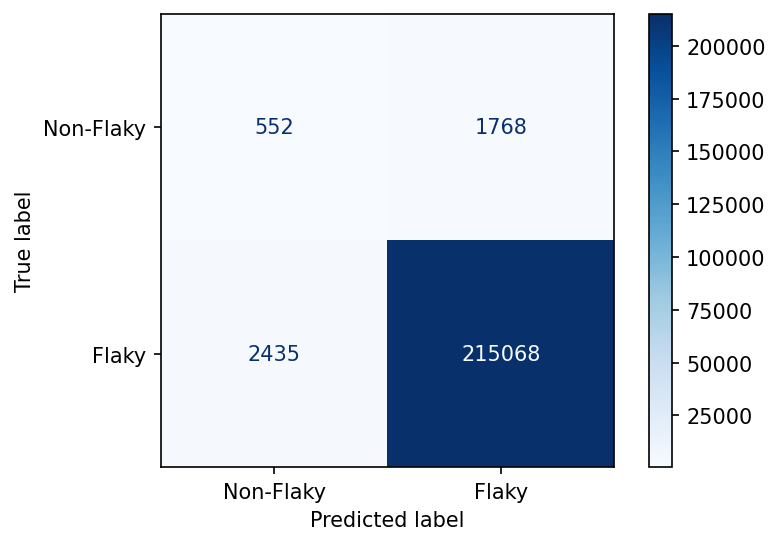
\includegraphics[width=0.6\textwidth]{figures/chromium/rq1.png}
\caption{Confusion matrix for the vocabulary-based model. High accuracy is reached similar to the performance reported in previous works. Nonetheless, 1,768 (76.2\%) out of the 2,320 fault-triggering failures are mislabeled as flaky.}
\label{fig:confMatrix}
\end{figure}

The confusion matrix of our model decisions is depicted in Figure ~\ref{fig:confMatrix}. The x-axis reports the predicted label and the y-axis the actual label. Correct classifications are displayed in the top left (TN) and bottom right (TP). We clearly observe that the model is able to detect flaky tests with high precision. We also see that 2,435 flaky tests are classified as non-flaky (FN). This number is also important to consider: it translates in all cases where developers will be required to investigate irrelevant failures.

We want to further understand the reasons behind the classification of fault-triggering failures. Therefore, we analyse the (fault-revealing) tests causing those failures. Out of the 2,320 fault-triggering failures, 1,768 are in the set of false positives (76.2\%) among which we found 463 (20\% of all fault-triggering failures) whose tests have a history of flakiness (flakeRate > 0) and 1,305 (56.2\% of all fault-triggering failures) without flakiness history. Here it must be noted that depending on the size of the history considered, we may have more tests with past flakiness or less. Overall in our data, 1/3 of all fault-triggering failures are due to tests that have exhibited flakiness behaviour. 

\begin{tcolorbox}[
    left=2pt,right=2pt,top=2pt,bottom=2pt,
    arc=0pt,
    boxrule=1.2pt
]
\textbf{RQ1:} Similar to previous studies, we report accurate predictions when aiming at flaky tests. However, a high proportion (76.2\%) of all fault-triggering failures is classified as flaky (missed faults) and still an important number (2,435) of flaky tests are marked as fault-triggering failures (false alerts).
\end{tcolorbox}

\subsection{RQ2: Discerning flaky from fault triggering test failures when training on test failures}

The results from RQ1 show that a vocabulary-based model trained to detect flaky tests would still yield an important number of missed faults and false alerts despite having high accuracy. Thus, our goal with RQ2 is to check whether by training our vocabulary-based model we can improve the performance of recognising fault-triggering failures. 

Table ~\ref{table:rq2and3} reports the results of such a model. In particular, the first row reports results based on failure training while the second row reports results related to RQ3. Similar to RQ1, we see a high precision and recall, 99.7\% and 91.3\% respectively, when predicting flaky failures. More interestingly, the MCC slightly increased to 0.25. 

\begin{tcolorbox}[
    left=2pt,right=2pt,top=2pt,bottom=2pt,
    arc=0pt, 
    boxrule=1.2pt
]
\textbf{RQ2:} When training on test failures, solely relying on test code vocabulary as features, to predict if a test failure is flaky or fault-triggering, model performance slightly improves but is still not effective in the context of the Chromium CI.
\end{tcolorbox}

\begin{table}[ht]
\caption{Vocabulary-based model performance for the prediction of \textit{flaky failures vs fault-triggering failures} when training on flaky vs non-flaky (fault-triggering and passing test executions). The approach does not work when solely relying on static features (\ie the test source code) and is improved when considering execution features.}
\label{table:rq2and3}
\centering
\begin{tabular}{c|c|c|c|c} 
 \toprule
 \textbf{Execution features} & \textbf{Precision} & \textbf{Recall} & \textbf{MCC} & \textbf{FPR} \\ [0.5ex] 
 \midrule
 No & 99.7\% & 91.3\% & 0.25 & 20.3\%\\ 
 Yes & 99.5\% & 98.7\% & 0.42 & 42.3\%\\ 
 \bottomrule
\end{tabular}
\end{table} 


\subsection{RQ3: Improving the accuracy of the flaky test failure predictions}

In this RQ we check the performance of the vocabulary-based models on the failure classification task when considering additional features from the test executions (run duration, and tests' historical flake rate). These features reflect better the characteristics of the test executions and are linked with test flakiness thereby leading to better results. 

In particular, the second row of Table~\ref{table:rq2and3} reports the related performance. We observe an improvement compared to the model that relies only on vocabulary (RQ2). This new model achieves a similar precision and recall of 99.5\% and 98.7\% and an improved MCC value 0.42, indicating a better performance in comparison to randomly picked selections. We see that the FPR increased to 42.3\%. Together, the results can be explained by fewer false alerts: flaky failures being marked as fault-triggering by the model. 

\begin{tcolorbox}[
    left=2pt,right=2pt,top=2pt,bottom=2pt,
    arc=0pt,
    boxrule=1.2pt
]
\textbf{RQ3} When equipped with execution-related features, the vocabulary-based prediction methods do a better job of distinguishing flaky failures from fault-triggering failures (0.42 MCC). Still, the need remains for dedicated methods to successfully learn this challenging classification task.
\end{tcolorbox}